\chapter{Standard Model}
\label{chap:sm}
The \ac{SM} of particle physics is a quantum field theory that describes all
known fundemental constituents of matter and their interactions through the
strong, weak and electromagnetic forces.

The theory is based on the $SU(3)_c \otimes SU(2)_L \otimes U(1)_Y$ gauge
group.

This chapter reviews the \ac{SM} of particle physics. The first section will 
introduce the two families of elementary matter particles, the leptons and quarks,
 and the latter section will then summarise the theoretical background
to the standard model.

The theory was pieced together in the 60s and 70s and comprises two families of
elementary particles, called quarks and leptons, and incorporates the theories
of quantum electrodynamics (QED), Glashow-Weinberg-Salam theory of electroweak
dynamics and quantum chromodynamics (QCD).

The Standard Model is remarkable in its accuracy, describing every experimental
test performed.  
\todo[inline]{MAKE THIS GOODER.}

\section{Constituents of the Standard Model}
\label{sec:matter}
Within the Standard Model matter is described as being constructed from a small
number of spin$=\nicefrac{1}{2}$ particles called fermions that interact with
the electromagnetic, weak and strong forces. The fermions are divided in to two
families called, leptons and quarks, according to their experimentally measured
properties such as their charge. 
Each family of fermions can be further subdivided in to three generations that
increase progressively increase in mass. The fermions of the Standard Model and
some of their properties are summarised in \TableRef{tab:particles}.

\begin{table}[htbp]
\begin{center}
\begin{tabular}{ l l l l l l }
\toprule
& 1st gen. & 2nd gen. & 3rd gen. & $Q$ & colour \\ 
\midrule
\multirow{2}{*}{quarks} 
& \Pup   & \Pstrange & \Ptop & $\nicefrac{+2}{3}$ & \multirow{2}{*}{RGB} \\
& \Pdown & \Pcharm   & \Pbottom & $\nicefrac{+2}{3}$ & \\ 
\multirow{2}{*}{leptons} 
& \Pnue      & \Pnum  & \Pnut & $0$ & \multirow{2}{*}{-} \\
& \Pelectron & \Pmuon & \Ptau & $1$ & \\ 
\bottomrule
\end{tabular}
\caption{The fermions of the Standard Model.}
\end{center}
\label{tab:particles}
\end{table}\todo{add particle masses?}

\subsection{Leptons}
Each lepton generation contains a charged lepton and a corresponding light
neutral particle called a neutrino. All leptons interact via the weak force,
whereas only the charge lepton interacts with the electromagnetic force.  The
first generation of leptons is the most familiar containing the electron and the
electron neutrino.

\subsection{Quarks}
Unlike leptons, quarks carry fractional charge, within each generation there is
a quark with a charge of $\nicefrac{2}{3}$ and another with a charge of
$\nicefrac{-1}{3}$. As well as the electric charge, quarks carry an additional
charge called the colour charge. The colour charge allows the quarks to interact
via the strong force in addition the electromagnetic and the weak forces.
The first generation of quarks is again the most familiar, containing the up and
down type quarks that are the constituents of the proton and neutron, which in
turn, with the electron, form atoms and all familiar matter.

\todo[inline]{antiparticles}

The heavier generations of quarks (strange, charm, bottom and top, or \Pstrange,
\Pcharm, \Pbottom and \Ptop) are unstable and decay eventually to \Pup or
\Pdown.
The heavy leptons, muon (\Pmuon) and tau (\Ptau), decay in a similar manner to
the stable electron. 
Due to the instability of the heavier generations of fermions, they can only be
found in  cosmic rays, or produced in high energy physics experiments.

\section{Fundamental Forces}
\label{sec:forces}

There are, as far as is known, four fundemental forces of nature, the strong,
weak, electromagnetic and gravitational forces.
\TableRef{tab:forces} summarises the force in order of decreasing
strength\footnote{The strength quoted in the table is a rough approximation as
`strength' depends on the source and distance of a force\cite{griffiths}}

\begin{table}[htbp]
\begin{center}
\begin{tabular}{ l l l l }
\toprule
Force           & Strength   & Theory   & Mediator \\
\midrule
Strong          & $10^{0}  $ & \acl{QCD} & Gluon \\
Electromagnetic & $10^{-2} $ & \acl{QED} & Photon \\
Weak            & $10^{-13}$ & \acl{EWK} & \PW and \PZ \\
Gravitational   & $10^{-42}$ & General Theory of Relativity & Graviton? \\
\bottomrule
\end{tabular}
\caption{The known four fundemental forces \cite{griffiths}.}
\end{center}
\label{tab:forces}
\end{table}

The \ac{SM} describes the strong, weak and electromagnetic interactions. Each
force is mediated by exchange of integer spin intermediate particles called
bosons.  Gravity is not included in the \ac{SM} as a complete quantum theory of
gravity has not yet been found. The gravitational force is so weak, when
compared to the other three forces its contribution to particle interactions is
negligable.

\subsection{Electromagnetic Force}
The classical theory for electromagnetism was formulated by Maxwell over a
centuary ago\cite{maxwell}, and a quantum theory of electrodynamics was
realised by Tomonaga, Feynman and Schwinger in the 1940s \cite{qed}.

The \ac{EM} force is the force that is responsible for interaction between
charged particles. The force is mediated by the massless photon, which means
that the \ac{EM} force is effective over infinite range.
The fundemetal process of \ac{QED} is shown in \FigureRef{fig:qed}.
\begin{figure}[htbp]
  \centering
  %
\includegraphics[width=0.5\textwidth]{placeholder}
  \missingfigure{elementary process for qed}
  \caption{The elementary process for \ac{QED} that all electromagnetic
interactions can be reduced to.}
  \label{fig:qed}
\end{figure}

The fine structure constant, $\alpha$, specifys the strength of the interaction
between charged particles and photon and is given by
\begin{equation}
\alpha = \frac{e^2}{4 \pi} \approx \frac{1}{137}
\end{equation}

The symmetry group for the electromagnetic interaction is $U(1)$. 

\subsection{Strong Force}

The strong force is the force responsible for the interaction between particles
that carry a colour charge, quarks and gluons. Unlike the electric charge, the
colour charge can have three posible values, conventionally called `red',
`green' and `blue' , as well as the corresponding anti colout charges
`anti-red', `anti-green' and `anti-blue'.
The fundemetal quark-gluon process of the strong force is shown in
\FigureRef{fig:qcd}.
\begin{figure}[htbp]
  \centering
  %
\includegraphics[width=0.5\textwidth]{placeholder}
  \missingfigure{elementary process for qcd}
  \caption{The quark-gluon vertex for \ac{QCD} .}
  \label{fig:qcdquark}
\end{figure}
The strong force is mediated by eight massless gluons which themselves carry
colour charge. This allows the gluons to self-interact which results gluon-gluon
vertexes in addtion to the quark-gluon vertex.
\begin{figure}[htbp]
  \centering
  %
\includegraphics[width=0.5\textwidth]{placeholder}
  \missingfigure{elementary process for qcd}
  \caption{The gluon-gluon vertices for \ac{QCD} .}
  \label{fig:qcdgluon}
\end{figure}

The coupling constant for the strnog force, $\alpha_s$, is given by,
\begin{equation}
\alpha = \frac{g_s^2}{4 \pi} \approx 1
\end{equation}
which is approximately 100 times stronger than the \ac{EM} force.
As the energy of the interaction increases the strength of the strong coupling
decreases. This is known as asymptotic freedom, at high-energy experiments
quarks appear to behave almost as free particles. However, at lower energies 
the coupling increases and quarks only appear in bound states, this is known as
quark confinement.
\todo{diagram of quark confinement here?}

The symmetry group for the strong force is $SU(3)$. 

\subsection{Weak Force}
The weak interaction occurs between all fermions and is the interaction
responsible in the radioactive decay of sub-atomic particles.  Unlike the strong
and electromagnetic forces, the weak force is mediated by the exchange of
massive particles, the \PWpm and \PZ bosons, which causes the weak interaction
to have a very short range.

There are two kinds of weak interactions: charged and neutral, mediated by the
\PW and the \PZ respectivly.

The fundemental vertex for the neutral vertex is shown in
\FigureRef{fig:neutral}, where the \PZ interacts with any quark or lepton.
The \pZ can mediate any process that can be mediated by the photon as well as
processes involving neutrinos.
\begin{figure}[htbp]
  \centering
  %
\includegraphics[width=0.5\textwidth]{placeholder}
  \missingfigure{elementary process for neutral weak}
  \caption{The fundemental vertex of neutral weak vertex.}
  \label{fig:neutral}
\end{figure}

The fundemental vertices for the charged current are shown in
\FigureRef{fig:charged}. The charged current has the unique ability to chage the
flavour of quarks and leptons by the exchange of \PW bosons. The charged current
will only interact with fermions of the same generation
(\HepProcess{\Pelectron\to\Pnue} but never
\HepProcess{\Pelectron\to\Pnum}).
\begin{figure}[htbp]
  \centering
  %
\includegraphics[width=0.5\textwidth]{placeholder}
  \missingfigure{elementary process for neutral weak}
  \caption{The fundemental vertex of neutral weak vertex.}
  \label{fig:charged}
\end{figure}

The weak interaction also violates parity ($P$) and charge conjugation ($C$). A
well known example of parity violation in weak interactions is the Wu experiment
\cite{wu}. In the experiment the $\beta$ decay of nuclei (Cobalt-60) polarised by an
external magnetic is studied, 
\begin{equation}
\begin{matrix}
\Rightarrow\Rightarrow \\
^{60}\mathrm{Co} \\
~   
\end{matrix}
\to
{^{60}\mathrm{Ni}}
+
\begin{matrix}
\Rightarrow \\
\Pelectron \\
\leftarrow 
\end{matrix}
+
\begin{matrix}
\Rightarrow \\
\APnue \\
\rightarrow 
\end{matrix}
\end{equation}
The Cobalt-60 nuclei are aligned to the external magnetic field. By conservation
of angular momentum, the neutrino and electron spins must be parallel and
aligned with the magnetic field. By
momentum conservation, the electron and neutrino must be produced in opposite
directions which means that the electron and neutrino must have oposite helicity. 
By changing the direction of the magnetic field, the system undergoes a parity
transformation
\begin{equation}
\begin{matrix}
\Leftarrow\Leftarrow \\
^{60}\mathrm{Co} \\
~   
\end{matrix}
\to
{^{60}\mathrm{Ni}}
+
\begin{matrix}
\Leftarrow \\
\Pelectron \\
\leftarrow 
\end{matrix}
+
\begin{matrix}
\Leftarrow \\
\APnue \\
\rightarrow 
\end{matrix}
\end{equation}
If parity is conserved then the electron would have no preference in direction.
However, what was seen was that the electron was preferentially emitted in the
oppsoite direction to their spin, the weak interaction exhibits maximal parity
violation.
More generally, the \PWpm boson is unique in that it only interacts with left handed
particles (or right handed antiparticles).

The \PW and \PZ bosons also have 3 and 4 vertex couplings to each another.

\section{Theoretical Background}
\label{sec:forces}
This section will introduce some of the ideas that drive the
theoretical background to the Standard Model.
The first section will give a brief overview on symmetries in physics and how
they can dictate particle interactions. In \SectionRef{sec:QED}, quantum
electrodynamics is introduced along with the idea of local gauge invariance.
\SectionRef{sec:EWK} details the weak interaction and the unification of the weak 
and the electromagnetic forces. \SectionRef{sec:higgs} describes the Higgs mechanism
which introduces the masses of the gauge bosons and fermions via spontaneous
symmetry breaking. The \SectionRef{sec:QCD} summarises the quantum
chromodynamics theory that describes the strong force.

\subsection{Symmetry and Groups}
\label{sec:symmetry}
Noether's theorem states that for every symmetry of nature, there is
a corresponding quantity that is conserved and conversely each conservation law
is the result of some underlying symmetry.
\todo[inline]{this whole section is horrible}

For example, the laws of physics are symmetrical with respect to translations in
time and space, and this leads directly to conservation of energy and momentum
respectively. Other symmetries and conservation laws are summarised in
\TableRef{tab:symmetry}

\begin{table}[htbp]
\begin{center}
\begin{tabular}{ l l }
Symmetry & Conserved Quantity \\ \hline
Time     & Energy \\
Space    & Momentum \\
Rotation & Angular Momentum \\
Gauge    & Electric Charge \\
\end{tabular}
\caption{Examples of symmetries and their corresponding conservation laws.
\label{tab:symmetry}}
\end{center}
\end{table}

It is currently believed that all particle interactions are dictated by symmetry
principles.  In group theory symmetry operations, such as rotations, can be
described by mathematical groups.
The most common groups to physics are unitary groups, $U(n)$, which are the
collection of all the $n\times n$ unitary ($U^{-1} = \tilde{U}^{*}$) matrices, and
the special unitary groups, $SU(n)$, which have the additional requirement that
the matrices have a determinant of 1.

\subsection{Quantum Electrodynamics}
\label{sec:QED}
In quantum electrodynamics, QED, an electron can be described as a complex
field, $\psi$. The Lagrangian is given by
\begin{equation}
\mathcal{L} = i \bar{\psi} \gamma_{\mu} \partial^{\mu} \psi - m \bar{\psi}\psi .
\end{equation}
This Lagrangian is invariant under a `global' phase transformation,
\begin{equation}
\psi(x) \to e^{i\alpha} \psi(x),
\label{eq:global}
\end{equation}
where $\alpha$ is a global arbitrary parameter. The Lagrangian is said to exhibit
global gauge invariance. The family of transformations, $R =
e^{i \alpha}$, where $\alpha$ is real and continuous, forms the unitary
Abelian \footnote{Abelian refers to the property that all the elements in a
group commute, $R(\alpha)R(\beta) = R(\beta)R(\alpha)$.}
group $U(1)$. 
More generally, the \EquationRef{eq:global} can be rewritten as,
\begin{equation}
\psi(x) \to e^{i\alpha(x)} \psi(x),
\label{eq:local}
\end{equation}
where $\alpha$ is now a function of the space time coordinate $x$. This is known
as a local phase transformation. Unfortunately, under this transformation, the
Lagrangian is no longer invariant. This can be overcome by defining the
covariant derivative as,
\begin{equation}
D_{\mu} \equiv \partial_{\mu} - i e A_{\mu},
\end{equation}
where an additional vector field $A_{\mu}$ has been added, that transforms as 
\begin{equation}
A_{\mu} \to A_{\mu} + \frac{1}{e} \partial_{\mu} \alpha,
\end{equation}
and the new Lagrangian then becomes
\begin{equation}
\mathcal{L} = 
\bar{\psi}(i\gamma^{\mu}\partial_{\mu} - m)\psi + 
e \bar{\psi} \gamma^{\mu} A_{\mu} \psi - 
\frac{1}{4} F_{\mu\nu} F^{\mu\nu}. 
\end{equation}
The additional vector field, $A_{\mu}$, couples with the electron,
 and can be identified as the physical photon field. The additional
term, $\frac{1}{4} F_{\mu\nu} F^{\mu\nu}$, is the kinetic energy of the photon
field. Local gauge invariance has been restored with the introduction of the photon
field. An interesting result is that the photon is required to be massless, as the introduction of
a mass term for the photon, for example a term $\propto A_{\mu}A^{\mu}$,
similar to the mass term in the original Lagrangian, breaks
the gauge invariance.

\subsection{Weak interaction and Electroweak Unification}
\label{sec:EWK}

The weak force can be examined in a similar way to QED, but with the non-Abelian
$SU(2)$ symmetry group. The weak force distinguished between the chirality, or
handedness, of a particle.
The handedness of a particle can be incorporated by introducing an additional
quantum number called the weak isospin, $I$.
For a left-handed fermion, $I=\nicefrac{1}{2}$ and the third component,
\begin{equation}
I_{3} =
  \begin{cases}
    \frac{1}{2}  & \text{for \Pnulepton}_L,  \\
    \frac{-1}{2} & \text{for \Plepton}_L, \\
    0            & \text{for \Plepton}_R.
  \end{cases}
\end{equation}
The isospin, hypercharge ($Y$) and electric charge ($Q$) can be related with the
Gell-Mann-Nishijima relation,
\begin{equation}
Q = I^{3} + \frac{1}{2}Y.
\end{equation}

The electromagnetic and weak coupling constants are not independent, the means that it is
possible to have a unified description of both the electromagnetic and weak
forces. This is known as electroweak (EWK) unification.

The electromagnetic and weak force can be described with a single group,
\begin{equation}
SU(2)_{L} \times U(1)_{Y},
\end{equation}
which is the cross product of the $SU(2)$ and $U(1)$ groups. The $L$ subscript
indicates the left handed components only and the $Y$ refers to the hypercharge.

In a similar manner to how requiring U(1) local gauge invariance led to insights
in to the QED Lagrangian, by requiring $SU(2)_{L} \times U(1)_{Y}$ local gauge
invariance it will be possible to infer information on the EWK Lagrangian.
The EWK Lagrangian can be written as the sum of many parts,
\begin{equation}
\mathcal{L}_{EWK} = 
\mathcal{L}_{fermion}
+ \mathcal{L}_{gauge}
+ \mathcal{L}_{scalar}
+ \mathcal{L}_{yukawa}.
\end{equation}
The first two terms have analogues with the QED case where as the second two
terms will be introduced with the Higgs mechanism.

The fermion term has a lepton and a quark part.
\begin{equation}
\mathcal{L}_{fermion} =
 \mathcal{L}_{lepton}
+ \mathcal{L}_{quark}.
\end{equation}
In this description the left handed fermions form isospin doublets and the right
handed fermions are singlets. For the case of the leptons $l_{L}$ is a left
handed doublet,
\begin{equation}
l_{L} = \left( \begin{matrix} \nu \\ e \end{matrix} \right)_{L},
\end{equation}
and $e_{R}$ is a right handed singlet.
For the case of the quarks, $q_{L}$ is a left handed doublet,
\begin{equation}
q_{L} = \left( \begin{matrix} u\\ d \end{matrix} \right)_{L},
\end{equation}
and there are two right handed singlets, the $u_{R}$ and the $d_{R}$.
The quark and lepton Lagrangians can be written,
\begin{align*}
\mathcal{L}_{lepton} &= 
\bar{l_{L}} i \gamma^{\mu} D_{\mu} l_{L} +
\bar{e_{R}} i \gamma^{\mu} D_{\mu} e_{R}, \\
\mathcal{L}_{quark} &= 
\bar{q_{L}} i \gamma^{\mu} D_{\mu} q_{L} +
\bar{u_{R}} i \gamma^{\mu} D_{\mu} u_{R} +
\bar{d_{R}} i \gamma^{\mu} D_{\mu} d_{R},
\end{align*}
where the covariant derivative has been introduced,
\begin{equation}
D_{\mu}
= (\partial_{\mu} 
- ig \mathbf{T} \cdot \mathbf{W}_{\mu}
+ \frac{ig\prime}{2} Y B_{\mu} ) ,\\
\end{equation}
where $g$ and $g\prime$ are the coupling constants for the group,
$\mathbf{T}=\mathbf{\tau}/2$ for left-handed particles and 
$\mathbf{T}=0$ for right-handed and $\mathbf{\tau}$
are the generators for the $SU(2)$ group. A total of four gauge fields have been
introduced; three fields, $\mathbf{W}_{\mu}$ , corresponding to the $SU(2)_{L}$
group and a single gauge field, $B_{\mu}$ corresponding to the $U(1)_{Y}$ group.
The physical $\PWp$ and $\PWm$ bosons are superpositions of the $W^{1}_{\mu}$
and $W^{2}_{\mu}$ gauge fields
\begin{equation}
W^{\pm}_{\mu} = \frac{1}{\sqrt{2}} \left(W^{1}_{\mu} \mp W^{1}_{\mu}\right),
\label{eq:wgauge}
\end{equation}
and the photon and Z boson are combinations of the $B_{\mu}$ and $W^{3}_{\mu}$
gauge fields,
\begin{equation}
\left( \begin{matrix} A_{\mu}\\ Z_{\mu}\end{matrix}\right) =
\left( \begin{matrix} \cos\theta_{W} && \sin\theta_{W} \\  
                      -\sin\theta_{W} && \cos\theta_{W} \end{matrix}\right) 
\left( \begin{matrix} B_{\mu}\\ W^{3}_{\mu}\end{matrix}\right) ,
\label{eq:bgauge}
\end{equation}
where $\theta_{W}$ is the Weinberg angle which is related to the coupling
constants by
\begin{align*}
\sin\theta_{W} &= \frac{g\prime}{\sqrt{g^{2}+g\prime^{2}}},\\
\cos\theta_{W} &= \frac{g}{\sqrt{g^{2}+g\prime^{2}}}.
\end{align*}
\todo{comment on how the covariant derivative is different for L and R}

The gauge part of the Lagrangian contains the kinetic terms and self interaction
terms for the gauge fields,
\begin{equation}
\mathcal{L}_{gauge} = 
- \frac{1}{4} \mathbf{W}_{\mu\nu} \cdot \mathbf{W}^{\mu\nu}
- \frac{1}{4} B_{\mu\nu} B^{\mu\nu},
\end{equation}
where
\begin{align*}
\mathbf{W}_{\mu\nu} &=
\partial_{\mu} \mathbf{W}_{\nu} -
\partial_{\nu} \mathbf{W}_{\mu} +
g \mathbf{W}_{\mu} \times \mathbf{W}_{\nu}\\
B_{\mu\nu} &= 
\partial_{\mu} B_{\nu}-
\partial_{\nu} B_{\mu}.
\end{align*}
The last term of $\mathbf{W}_{\mu\nu}$ is required to keep the Lagrangian invariant
under the non-Abelian gauge transformation of the $SU(2)$ group. The term
introduces cubic and quadratic terms in to the Lagrangian that describe the 3 and 4
vertex interactions of the gauge boson.
\todo{diagram of these vertexes?}

\subsection{Higgs Mechanism}
\label{sec:higgs}
The Lagrangian, as it has been written so far, does not include terms for the
mass of any of the particles. 
Adding in mass terms by hand will break the
gauge symmetry rendering the theory meaningless. The symmetry needs to be broken
in some natural way.
The Higgs mechanism is a mechanism which introduces the mass terms by
spontaneous symmetry breaking.

The Higgs mechanism introduces four real scalar fields, that can be arranged in a
isospin doublet,
\begin{equation}
\Phi = \left( \begin{matrix} \phi^{+} \\ \phi^{0} \end{matrix} \right),
\end{equation}
where,
\begin{align*}
\phi^{+} &=\frac{1}{\sqrt{2}} (\phi_{1} + i \phi_{2}),\\
\phi^{0} &=\frac{1}{\sqrt{2}} (\phi_{3} + i \phi_{4}).
\end{align*}

The scalar part of the Lagrangian is
\begin{equation}
\mathcal{L}_{scalar} = 
\left(D^{\mu}\phi\right) \left(D_{\mu}\phi\right) - V(\phi),
\end{equation}
where the potential is,
\begin{equation}
V(\phi) = 
\mu^{2}\phi^{\dagger}\phi + 
\lambda^{2} \left( \phi^{\dagger} \phi \right)^{2},
\end{equation}
where $\lambda$ and $\mu$ are free parameters. Choosing  $\lambda>0$ and
$\mu^{2}<0$ there is a minima at,
\begin{equation}
\phi^{\dagger} \phi = \frac{- \mu^{2}}{2 \lambda}.
\end{equation}

\begin{figure}[htbp]
  \centering
  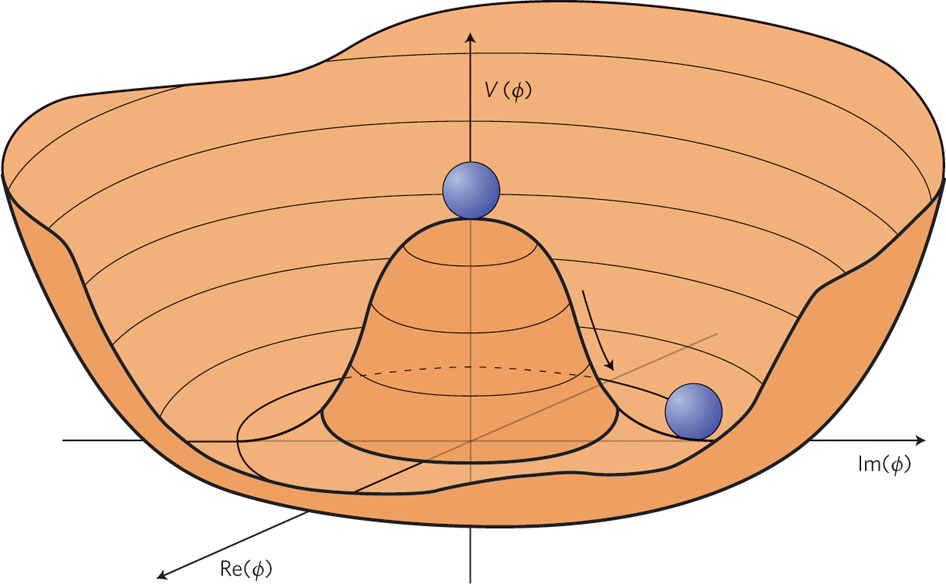
\includegraphics[width=0.7\textwidth]{nphys1874-f1.jpg}
  \caption{ The Higgs potential, $V(\phi)$, in the form of a 'Mexican hat',
leads to spontaneous symmetry breaking, from \cite{}}
  \label{fig:higgspot}
\end{figure}

A plot of the Higgs potential with $\mu^{2}<0$ is shown in
\FigureRef{fig:higgspot}. It is unstable to small perturbations, and will fall
to a lower energy state. 
The ground state does not have the same symmetry as the Lagrangian, by
selecting a minima the symmetry has become broken. An example choice of minima
could be,
\begin{equation}
\phi_{1} = \phi_{2} = \phi_{4} = 0,
\end{equation}
and
\begin{equation}
\phi_{3} = \frac{-\mu^{2}}{\lambda} \equiv v^{2}.
\end{equation}
This choice of minima is motivated to ensure $U(1)_{EM}$ symmetry remains
unbroken and
that the photon is massless.
Substituting this vacuum expectation value,
\begin{equation}
\phi_{0} = \frac{1}{\sqrt{2}}\left(\begin{matrix}0\\v\end{matrix}\right),
\end{equation}
in to the Lagrangian, and using \EquationRef{eq:wgauge} and
\EquationRef{eq:bgauge}, additional terms are found\cite{},
\begin{equation}
\left(\frac{vg}{2}\right)^{2} W^{+}_{\mu} W^{- \mu}, 
\left(\frac{vg}{2}\right)^{2} \frac{1}{2\cos\theta_{W}} Z_{\mu} Z^{\mu},
\end{equation}
which appear to be mass terms for the gauge bosons.
The masses of the gauge bosons can be written as 
\begin{equation}
M_{W} = \frac{gv}{2}, 
M_{Z} = \frac{gv}{2\cos\theta_{W}}.
\end{equation}
There is no mass term for the photon (for example $A_{\mu}A^{\mu}$) so it
remains massless.

Another feature of the Higgs mechanism, is that it also provides a way to
introduce mass terms for the fermions, in a gauge invariant way, via the Yukawa
coupling between the leptons with the Higgs field. The Lagrangian for this
interaction can be written as, 
\begin{equation}
\mathcal{L}_{yukawa} = -G_{f}\bar{L}\phi R + h.c. \ ,
\end{equation}
where $G_{f}$ is the coupling to the Higgs field known as the Yukawa coupling
\begin{equation}
-G_{f} = \frac{\sqrt{2}m_{f}}{v}
\end{equation}
which is proportional to the mass of the fermion. 
\todo{summarise the main points of this section}

\subsection{Quantum Chromodynamics}
\label{sec:QCD}
The final piece of the puzzle is the strong interaction, described by quantum
chromodynamics, QCD. 
Quantum chromodynamics follows from similar reasoning to the QED case, but with
the Abelian $U(1)$ symmetry group replaced with the non-Abelian $SU(3)$ symmetry
group of transformations on the quark colour fields.

The local gauge phase transformation becomes,
\begin{equation}
q(x) \to e^{i\alpha_a(x)T_a} q(x),
\end{equation}
which breaks the invariance of the Lagrangian. Again this is overcome by
introducing the covariant derivative,
\begin{equation}
D_{\mu} \equiv \partial_{\mu} + i g T_{a} G_{\mu}^{a},
\end{equation}
where eight gauge fields have been introduced, instead of the single field in
QED. \todo{what is T} 
The gauge fields transform as,
\begin{equation}
 G_{\mu}^{a} \to G_{\mu}^{a} 
-\frac{1}{g}\partial_{\mu}\alpha_{a}]
-f_{abc}\alpha_{b}G^{c}_{\mu},
\end{equation}
where last additional term has been added is to produce a gauge invariant
Lagrangian due to the non-Abelian gauge transformation.

The final Lagrangian for QCD can now be written,
\begin{equation}
\mathcal{L} = 
\bar{q}(i\gamma^{\mu}\partial_{\mu} - m)q -
g \bar{q} \gamma^{\mu} G_{\mu}^{a} - 
\frac{1}{4} G_{\mu\nu}^{a} G^{\mu\nu}_{a},
\end{equation}
where the field strength tensor $G^{\mu\nu}_{a}$ is given by,
\begin{equation}
G^{\mu\nu}_{a} 
= \partial{\mu} G^{a}_{\nu}
- \partial{\nu} G^{a}_{\mu}
-g f_{abc} G^{b}_{\mu} G^{c}_{\nu}.
\end{equation}

In a similar way to QED, the Lagrangian for interacting coloured quarks, $q$, and
vector gluons, $G_{\mu}$, result from the simple requirement of local colour
phase invariance of the quark fields. Unlike the QED case, eight gauge fields
are needed due to the three quark colour fields.  Similar to QED, the gluons are
required to  be massless.

The field strength tensor, $G^{\mu\nu}_{a}$, introduces terms that are cubic and
quadratic in $G$. These represent three and four vertex gluon interactions that
are a results of the non Abelian nature of the $SU(3)$ group.
\todo{diagram of this?}

